% !TeX spellcheck = en_GB
% !TeX program = lualatex
%
% v 2.3  Feb 2019   Volker RW Schaa
%		# changes in the collaboration therefore updated file "jacow-collaboration.tex"
%		# all References with DOIs have their period/full stop before the DOI (after pp. or year)
%		# in the author/affiliation block all ZIP codes in square brackets removed as it was not %         understood as optional parameter and ZIP codes had bin put in brackets
%       # References to the current IPAC are changed to "IPAC'19, Melbourne, Australia"
%       # font for ‘url’ style changed to ‘newtxtt’ as it is easier to distinguish "O" and "0"
%
\documentclass[a4paper,
               %boxit,        % check whether paper is inside correct margins
               %titlepage,    % separate title page
               %refpage       % separate references
               %biblatex,     % biblatex is used
               keeplastbox,   % flushend option: not to un-indent last line in References
               %nospread,     % flushend option: do not fill with whitespace to balance columns
               %hyphens,      % allow \url to hyphenate at "-" (hyphens)
               %xetex,        % use XeLaTeX to process the file
               %luatex,       % use LuaLaTeX to process the file
               ]{jacow}
%
% ONLY FOR \footnote in table/tabular
%
\usepackage{pdfpages,multirow,ragged2e} %
%
% CHANGE SEQUENCE OF GRAPHICS EXTENSION TO BE EMBEDDED
% ----------------------------------------------------
% test for XeTeX where the sequence is by default eps-> pdf, jpg, png, pdf, ...
%    and the JACoW template provides JACpic2v3.eps and JACpic2v3.jpg which
%    might generates errors, therefore PNG and JPG first
%
\makeatletter%
	\ifboolexpr{bool{xetex}}
	 {\renewcommand{\Gin@extensions}{.pdf,%
	                    .png,.jpg,.bmp,.pict,.tif,.psd,.mac,.sga,.tga,.gif,%
	                    .eps,.ps,%
	                    }}{}
\makeatother

% CHECK FOR XeTeX/LuaTeX BEFORE DEFINING AN INPUT ENCODING
% --------------------------------------------------------
%   utf8  is default for XeTeX/LuaTeX
%   utf8  in LaTeX only realises a small portion of codes
%
\ifboolexpr{bool{xetex} or bool{luatex}} % test for XeTeX/LuaTeX
 {}                                      % input encoding is utf8 by default
 {\usepackage[utf8]{inputenc}}           % switch to utf8

\usepackage[USenglish]{babel}

%
% if BibLaTeX is used
%
\ifboolexpr{bool{jacowbiblatex}}%
 {%
  \addbibresource{jacow-test.bib}
  \addbibresource{biblatex-examples.bib}
 }{}
\listfiles

%%
%%   Lengths for the spaces in the title
%%   \setlength\titleblockstartskip{..}  %before title, default 3pt
%%   \setlength\titleblockmiddleskip{..} %between title + author, default 1em
%%   \setlength\titleblockendskip{..}    %afterauthor, default 1em

\begin{document}

\title{CI-CD Practices with the TANGO-controls framework in the context of the Square Kilometre Array (SKA) Telescope Project\thanks{Work supported by Italian Government (MEF - Ministero dell'Economia e delle Finanze, MIUR - Ministero dell'Istruzione, dell'Università e della Ricerca)}}

\author{M. Di Carlo\thanks{matteo.dicarlo@inaf.it}, INAF Osservatorio Astronomico d'Abruzzo, Teramo, Italy \\
		M. Bartolini, SKA Organisation, Macclesfield, UK \\
		K. Madisa, A. J. Venter, A. de Beer, SKA South Africa, Cape Town, South Africa \\
		J. B. Morgado, D. Bartashevich, D. Nunes, Instituto de Telecomunicações (GRIT) \\ 
		Universidade de Aveiro, Portugal}
\maketitle

%
\begin{abstract}
  The Square Kilometre Array (SKA) project is an international effort to build two radio interferometers in South Africa and Australia to form one Observatory monitored and controlled from the global headquarters (GHQ) based in the United Kingdom at Jodrell Bank. The project is now approaching the end of its design phase and gearing up for the beginning of formal construction. The period between the end of the design phase and the start of the construction phase, has been called bridging and, one of its main goals is to promote some CI-CD practices among the software development teams. CI-CD is an acronym that stands for continuous integration and continuous delivery and/or continuous deployment. Continuous integration (CI) is the practice to merge all developers local (working) copies into the mainline very often (many times per day). Continuous delivery is the approach of developing software in short cycle ensuring that it can be released anytime and continuous deployment is the approach of delivering the software frequently and automatically. The present paper wants to analyse the decision taken by the system team (a specialized agile team devoted to developing and maintaining the tools that allows continuous practises) in order to promote the CI-CD practices with TANGO controls framework. 

\end{abstract}

\section{Introduction}
When creating releases for the end-users, every big software industry faces the problem of integrating the different parts of the software and bring them to the production environment, that is where users work. The problem arises when many parts of the project are developed independently for a period of time and when merging them into the same branch, the process takes more than what was planned. In a classical waterfall software development process this is usual, but the same happens also following the classical git flow, also known as feature-based branching, that is when a branch is created for a particular feature. Considering, for example, one hundred developers working in the same repository each of them creating one or two branches, then it is easy to understand what is called the “merge hell” that is when every merge has to deal with conflict parts and it is impossible, for a single developer, to solve all the conflicts thus creating delay in publishing any release. 
This problem was analyses at the Square Kilometre Array (SKA) project, an international effort to build two radio interferometers in South Africa and Australia to form one Observatory monitored and controlled from the global headquarters (GHQ) based in the United Kingdom at Jodrell Bank.  
The selected development process is Agile (Scaled Agile framework) that is basically incremental and iterative with a specialized team (known as system team) devoted to support the continuous Integration, test automation and continuous Deployment.


\section{TANGO-controls overview}
One of the most important decisions taken by the SKA project is the adoption of the TANGO-controls framework which is a middleware for connecting software processes together mainly based on the CORBA standard (Common Object Request Broker Architecture). The standard defines how to exposes the procedures of an object within a software process with the RPC protocol (Remote Procedure Call).  The TANGO framework extends the definition of object with the concept of Device which represents a real or virtual device to control that expose commands (that are procedures), attributes (like the state) and allows both synchronous and asynchronous communication with events generated from the attributes (for instance a change in the value can generate an event). Fig.~\ref{fig:tangodatamodel}  shows a module view of the framework.

\begin{figure}[!htb]
   \centering
   \includegraphics*[width=1\columnwidth]{SimplifiedDataModel}
   \caption{TANGO-Controls simplified data model.}
   \label{fig:tangodatamodel}
\end{figure}

\section{Continuous Integration (CI)}
CI refers to a set of development practices that requires developers to integrate code into a shared repository several times a day. Each check-in is then verified by an automated build, allowing teams to detect problems early.
According to Martin Fowler~\cite{CI}, there are a number of best practices to implement to reach CI: 
\begin{Itemize}
    \item Maintain a single source repository (for each component of the system) and try to minimize the use of branching, in favor of a single branch of the project currently under development. 
    \item Automate the build (possibly build all in one command).
    \item Together with the build, it must run also tests so to make the software self-testing (testing is crucial in CI because all the benefits of it come only if the test suite is good enough).
    \item Every commit should build on an integration machine: the more the developers commit the better it is (common practice is at least once per day). In fact, this reduces the number of potential conflicts and once a conflict is found, since the change is small, the fix is easier (as a consequence if a build fails then it must be fixed immediately).
    \item Keep the build fast so that a problem in integration can be found quickly.
    \item Multi-stage deployment: every build software must be tested in different environments (testing, staging and so on).
    \item Make it easy for anyone to get the latest executable version: all programmers should start the day by updating the project from the repository.
    \item Everyone can see what’s happening: a testing environment with the latest software should be running.
\end{Itemize}

\section{Continuous delivery and Continuous deployment (CD)}
Continuous delivery~\cite{CD} refers to an extension of the CI that correspond to automating the delivery of new releases of software in a sustainable way. The release frequency can be decided according to the business requirement but the greatest benefit is reached by releasing as quickly as possible. 
The deployment has to be predictable and sustainable, no matter if it is a large-scale distributed system, a complex production environment, an embedded system, or an app. Therefore the code must be in a deployable state. Testing is one of the most important activities and it needs to cover enough of your codebase. 
While it is often assumed that frequent deployment means lower levels of stability and reliability in the systems, this is not the reality and, in general, in software the golden rule is “if it hurts, do it more often, and bring the pain forward” (~\cite{CD}, page 26).
There are many patterns for deployment such as the blue-green deployment (Fig.~\ref{fig:bluegreendeploy}, (~\cite{CD}, page 261)) and, in general, all of them are related somehow to the DevOps culture. According to ~\cite{DevOps}, "DevOps is the outcome of applying the most trusted principles from the domain of physical manufacturing and leadership to the IT value stream. [...] The result is world-class quality, reliability, stability, and security at ever lower cost and effort; and accelerated flow and reliability throughout the technology value stream, including Product Management, Development, QA, IT Operations, and Infosec". Practically it is an increased collaboration between development (intended as requirement analysis, development and testing) and operations (intended as deployment, operations and maintenance). In fact, it is very common, when those two areas are managed by different teams, that the development team loses interest in the operations aspects, when the software is managed by a different team. Having a shared responsibility means that development teams share the problems of operations by working together in automating deployment operations and maintenance. It is also very important that teams are autonomous: they should be empowered to deploy a change to operations with no fear of failures. 
Moreover, automation is one of the key elements in implementing a DevOps strategy, as it allows the teams to focus on what is valuable (code development, test result, etc. and not the deployment itself) and it reduces human errors.
\begin{figure}[!htb]
   \centering
   \includegraphics*[width=1\columnwidth]{BlueGreenDeploy}
   \caption{Blue-Green deployment: If the active environment in production is the blue box, it deploys on the green and if everything goes well the router can switch the incoming requests; if an error is discovered is always possible to rollback.}
   \label{fig:bluegreendeploy}
\end{figure}
The importance of those practices can be summarized in reducing risks of integration issues, of releasing new software and overall in having a better software product. 
Continuous deployment goes one step further as every single commit (!) to the software that passes all the stages of the build and test pipeline is deployed into the production environment. 

\section{Containerization}
The system engineering development process has been adopted in the initial design phase of the SKA project in order to reduce the complexity by dividing the project into simpler and easier to resolve elements. For every element of the system, an initial architecture has been developed, which comprises the software modules needed which requires a repository (each of them is a component of the system).
Since all components need to get deployed and tested together, the first decision taken is on how they need to be packaged.  A container is a standard unit of software that packages up code and all its dependencies so the component runs quickly and reliably across different computing environments. A Docker container image is a lightweight, standalone, executable package of software that includes everything needed to run an application: code (or more in general binary), runtime, system tools, system libraries and settings.
In order to allow all the teams to work in the same environment, it has been created a containerized Tango environment~\cite{SKA-docker} is summarized in Fig.~\ref{fig:skadocker}. 
\begin{figure}[!htb]
   \centering
   \includegraphics*[width=1\columnwidth]{ska-docker}
   \caption{SKA-docker project module view.}
   \label{fig:skadocker}
\end{figure}
Every tango project comes with a docker-composed based orchestration (docker-compose.yml file) that includes:
\begin{Itemize}
    \item MariaDB service container, 
    \item DatabaseDs service container,
    \item For each device server in the project, one container defined by the developer.
\end{Itemize}
Each container includes one application (in TANGO terms one device server) and testing is also made within a container (created on the fly) with a standardized (for SKA) metrics file output that states for each project/component the following information: 
\begin{Itemize}
    \item Build status: true or false,
    \item Test report,
    \item Coverage,
    \item Linting information.
\end{Itemize}
For the integration of all the docker images (coming from the different repositories), the integration environment is based on Kubernetes (k8s) orchestration~\cite{kubernetes} and Helm~\cite{helm}. Helm is a tool for managing Kubernetes charts where a chart is a package of pre-configured Kubernetes resources that are a set of information necessary to create an instance of a Kubernetes application. In specific every chart contains at least information concerning the version of the docker image and the pull policy for the orchestration. In specific every component has a helm chart that contains information concerning the version of the docker image and the pull policy for the orchestration. It also contains the needed information to initialize correctly the TANGO database (configuration of devices). Fig.~\ref{fig:k8sIntegrationRepo} summarize the module view of the structure of the repository for the integration of the SKA components. 
\begin{figure}[!htb]
   \centering
   \includegraphics*[width=1\columnwidth]{k8sIntegrationRepo}
   \caption{K8s Integration repository module view.}
   \label{fig:k8sIntegrationRepo}
\end{figure}

\section{Infrastructure}
The infrastructure described in this section is possible thanks to the use of a Makefile in each project that allows to simplify the work on containerization and, overall, the automation of the code building, testing and packaging processes. In fact, with one single command, it is possible to compile the project, generate the docker image and test it by dynamically creating a container for that purpose.  The Makefile also allows to push the docker image to the SKA repository. 
\subsection{Runtime view}
Fig.~\ref{fig:cicdInfra} describes the runtime view of the CICD infrastructure in place for the SKA project. The starting point is the source-code repository server where every team put their code (for instance it can be Github). The CICD Server requests the code from the source code repository periodically and keeps information about the execution of the pipeline (see next section).  The CI executor takes the pipeline configuration information and executes it pushing artifacts to the Artifacts repository. If tests are successful the executors starts the deployment of the software artifacts to various environments (like integration, stage and so on) using ansible scripts~\cite{ansible}.
\begin{figure}[!htb]
   \centering
   \includegraphics*[width=1\columnwidth]{cicdInfra}
   \caption{Runtime view of the SKA CI-CD infrastructure.}
   \label{fig:cicdInfra}
\end{figure}

\subsection{Data Entity}
The selected tool for CICD is Gitlab where the CI executor is called “runner” and the CICD server is a code repository that includes a description (in a yaml file) of the execution that has to be done by the runners. Gitlab includes also an artifacts repository called “pages” for each repository. Fig.~\ref{fig:datamodel} summarize the data model of the SKA CI-CD infrastructure in a UML diagram.
\begin{figure}[!htb]
   \centering
   \includegraphics*[width=1\columnwidth]{dataEntity}
   \caption{Data Model of the SKA CI-CD infrastructure.}
   \label{fig:datamodel}
\end{figure}

The entry point of the diagram is the Pipeline that is composed by many jobs. This has been standardised for each project in:
\begin{Itemize}
    \item Build, where code is compiled and a docker image is created;
    \item Linting, where code is analysed against a set (or multiple sets) of coding rules in order to check if it follows the best practices decided;
    \item Test, where the compiled package (and docker image) are tested; tests are grouped into Fast / Medium / Slow / Very Slow categories.
    \item Publish, where the coding artifacts are published;
    \item Pages, where test results and logs are published (the name comes directly by the Gitlab technology). 
\end{Itemize}

In the Gitlab cloud space the artifacts stored are the logs of each job executed and the test results obtained by the Test job. Other artifacts (python packages, docker images and so on) are stored in a different repository based on the Nexus tool. For each git revision there is a version of the pipeline configuration (stored in the repository with the name “.gitlab-ci.yml”). 


\section{Development workflow}
There are two possible workflow in order to make a change to a git repository whether there is branch or not. In general, two concepts are important to the SKA way of using GIT:
\begin{Itemize}
    \item The master branch of a repository shall always be stable.
    \item Branches shall be short lived, merging into master as often as possible.
\end{Itemize}

Stable means that the master branch shall always compile and build correctly, and executing automated tests with success. Every time a master branch results in a condition of instability, reverting to a condition of stability shall have precedence over any other activity on the repository.

Every commit triggers a pipeline build and there may be different rules applied to determine which stages are executed in the pipeline based on factors like the branch name. According to the data model, every pipeline job is associated with its git commit (including tag commits) and developers have to ensure that the stages complete as fast as possible. For this reason it is possible to parallelize jobs, for example unit tests and static analysis could be run in parallel. Developers needs to keep all tests working  on the “master” branch that must be kept stable.
When working on a development project, it is important to stick to these simple commit rules:
\begin{Itemize}
    \item Commit often.
    \item Git logs shall be human readable in sequence, describing the development activity.
    \item Use imperative forms in the commit message.
\end{Itemize}

\subsection{Workflow for master based development}
\begin{Itemize}
    \item A developer takes a copy of the current code base on which to work
    \item Work is started on a local copy
    \item As the developer advances in the implementation commits are done on the local git repo. 
    \item Unit tests are written and run in the development environment until successfully executed
    \item Once the tests pass the developer pushes the changes into a remote repository 
    \item The CI server 
\begin{Itemize}
    \item Checks out changes every X minutes (or when they occur)
    \item Runs static code analysis and provide feedback to the developers
    \item Builds the system 
    \item Runs all tests
    \item Releases deployable artefacts for testing (reports, code analysis, etc.)
    \item Assigns a build label to the version of the code it just built (i.e. docker image version)
    \item Alerts the team if the build or tests fail which fixes the issue asap
    \item Provide feedback about coverage metrics
\end{Itemize}
\end{Itemize}

\subsection{Workflow for story based branching }
\begin{Itemize}
    \item A developer takes a copy of the current code base on which to work
    \item Work is started on a new branch based on the story being implemented
    \item As  the developer advances in the implementation commits are done on the local git repo. 
    \item Unit tests are written and run in the development environment until successfully executed
    \item Once the tests pass the developer pushes the changes into a remote branch
    \item The CI server 
    \begin{Itemize}
        \item Checks out changes when they occur
        \item Runs static code analysis and provide feedback to the developer
        \item builds the system and runs unit and integration tests on the branch
        \item Provide feedback to the developer about test fail or success
        \item Provide feedback about coverage metrics
    \end{Itemize}
    \item Once all tests execute successfully on the branch, the developer makes a pull request for merging the changes into master.
    \item As part of the pull request the code is reviewed by other developers.
    \item Code is merged into master branch
    \item The CI server 
    \begin{Itemize}
        \item Runs all tests on the master branch
        \item Releases deployable artefacts for testing (reports, code analysis, etc.)
        \item Assigns a build label to the version of the code it just built (i.e. docker image version)
        \item Alerts the team if the build or tests fail which fixes the issue asap
    \end{Itemize}
\end{Itemize}

\section{Dashboard}
From a management point of view it is very important to monitor the projects in SKA with at least the following information: 
\begin{Itemize}
    \item Latest build status and date
    \item Latest green build date
    \item Test coverage
    \item Testing report
\end{Itemize}

In order to do that, a dashboard has been created as a progressive web app (PWA). this kind of web application are loaded like regular web pages or websites but can offer user functionalities such as working offline, push notifications, and device hardware access traditionally available only to native applications. In specific, PWAs combine the flexibility of the web with the experience of a native application. In particular progressive means that it works for every user, regardless of browser choice because they're built with progressive enhancement as a core tenet. Other important qualities are: 
\begin{Itemize}
    \item Responsive, it works for desktop, mobile, tablet;.
    \item Connectivity independent: it allows work offline
    \item App-like: feel like an app to the user with app-style interactions and navigation;
    \item Fresh: always up-to-date thanks to the service worker update process 
    \item Safe: HTTPS
\end{Itemize}

The deployment are based on a pipeline with two main jobs:
\begin{Itemize}
    \item Retrieve data, from Gitlab rest api download a set of json files (one per each page)
    \item Publish data, that generate the web page.
\end{Itemize}

\section{CONCLUSION}
All the decisions taken by the system team try to follow the continuous integration suggestion from Martin Fowler’s paper. In particular: 
\begin{Itemize}
    \item For each component of the system, there is only one repository with minimal use of branching that are short lived;
    \item The build of each component is automated together with tests that allows to push only the correct artifacts into the artifact repository;
    \item Every commit triggers a build in a different machine (not the local developer machine);
    \item Once the artifacts are built, they are transferred in an integration repository which run a kubernetes cluster and more tests are done;
    \item Having a common repository for the code artifacts and for the test results artifacts make it very easy to download the latest changes from every team and for each component;
    \item The integration environment is accessible for every developer. 
\end{Itemize}

There is some work still to be done, the first and most important is improving the performance of the tests. At the moment, tests are executed after the code is compiled and the docker images are built. A possible improvement is building the docker images after the tests are executed. Besides, more environments have to be created. For this purpose a kubernetes cluster is going to be used so that it will be possible to isolate each environment adding for each of them the specific resources needed in terms of GPUs or other resources. Having kubernetes will also make very easy to implement the blue-green deployment pattern.


\section{ACKNOWLEDGEMENTS}
This work has been made possible thanks to the financial support by the Italian Government (MEF - Ministero dell'Economia e delle Finanze, MIUR - Ministero dell'Istruzione, dell'Università e della Ricerca). This research is also supported by the project Enabling Green E-science for the SKA Research Infrastructure (ENGAGE SKA), reference POCI-01-0145-FEDER-022217, funded by COMPETE 2020 and FCT, Portugal.

%
% only for "biblatex"
%
\ifboolexpr{bool{jacowbiblatex}}%
	{\printbibliography}%
	{%
	% "biblatex" is not used, go the "manual" way
	
	%\begin{thebibliography}{99}   % Use for  10-99  references
	\begin{thebibliography}{9} % Use for 1-9 references
	
	\bibitem{TANGO-controls}
		TANGO-controls,
		\url{https://www.tango-controls.org/}
	
	\bibitem{CI}
		Martin Fowler, Continuous Integration,
		\url{https://martinfowler.com/articles/continuousIntegration.html}
		
	\bibitem{CD}
	    J. Humble, D. Farley, "Continuous Delivery: Reliable Software Releases Through Build, Test, and Deployment Automation",
	    2010, ISBN (0321601912, 9780321601919), Pub. Addison-Wesley Professional
	
	\bibitem{DevOps}
	    G. Kim, P. Debois, J. Willis, J. Humble, "The DevOps Handbook: How to Create World-Class Agility, Reliability, and Security in Technology Organizations", ISBN (1942788002 9781942788003)
	
	\bibitem{SKA-docker}
		SKA-docker repository,
		\url{https://gitlab.com/ska-telescope/ska-docker}
	
	\bibitem{kubernetes}
		kubernetes,
		\url{https://kubernetes.io}
			
	\bibitem{helm}
		Helm,
		\url{https://helm.sh}
		
	\bibitem{ansible}
	    Ansible, \url{https://www.ansible.com/}

	\end{thebibliography}
} % end \ifboolexpr
%
% for use as JACoW template the inclusion of the ANNEX parts have been commented out
% to generate the complete documentation please remove the "%" of the next two commands
% 
%%%\newpage

%%%%
% !TeX spellcheck = en_GB
%
\twocolumn[\vspace*{-1.8ex}\section{ANNEX A:\endgraf FORMATTING OF AUTHORS AND AFFILIATIONS}\vspace*{\baselineskip}]

\flushcolsend

The names of authors, their organizations/affiliations
and postal addresses should be grouped by affiliation and
listed in \SI{12}{pt} upper- and lowercase letters. The name of
the submitting or primary author should be first, followed
by the coauthors, alphabetically by affiliation. If the
author list for a given affiliation spans multiple lines,
please be sure to break the line in a manner that does not
split the author’s initials from the author’s last name. This
is easily done by placing unbreakable spaces between the
initials and last name. The affiliation name and address
are also best kept together on the same (but not necessarily
separate) line, wherever possible. (See, for example,
the entry for GSI in the following). In cases where authors
have multiple affiliations, the secondary affiliation is
inserted below the author/primary affiliation listing and is
indicated with a superscript, as shown in the following.


Footnotes on the title and author lines may be used for
acknowledgements and e-mail addresses, using a non-numeric
sequence of characters (\textsuperscript{*}, \textsuperscript{†},
\textsuperscript{‡}, \textsuperscript{§}, \textsuperscript{\P}
as generated by \LaTeX's \verb|\footnote| command).

For examples of the preferred formatting of authors and
affiliations, please consult the following list of JACoW
collaboration members.

For manuscripts submitted by large collaborations with
potentially many tens of authors and where, additionally,
there may be page number limitations, a format consisting
of the principle author’s name and institute, followed by
“on behalf of the \ldots\ collaboration”, is preferred.


\clearpage
%
% Include the title/author page of the JACoW Coolaboration
%
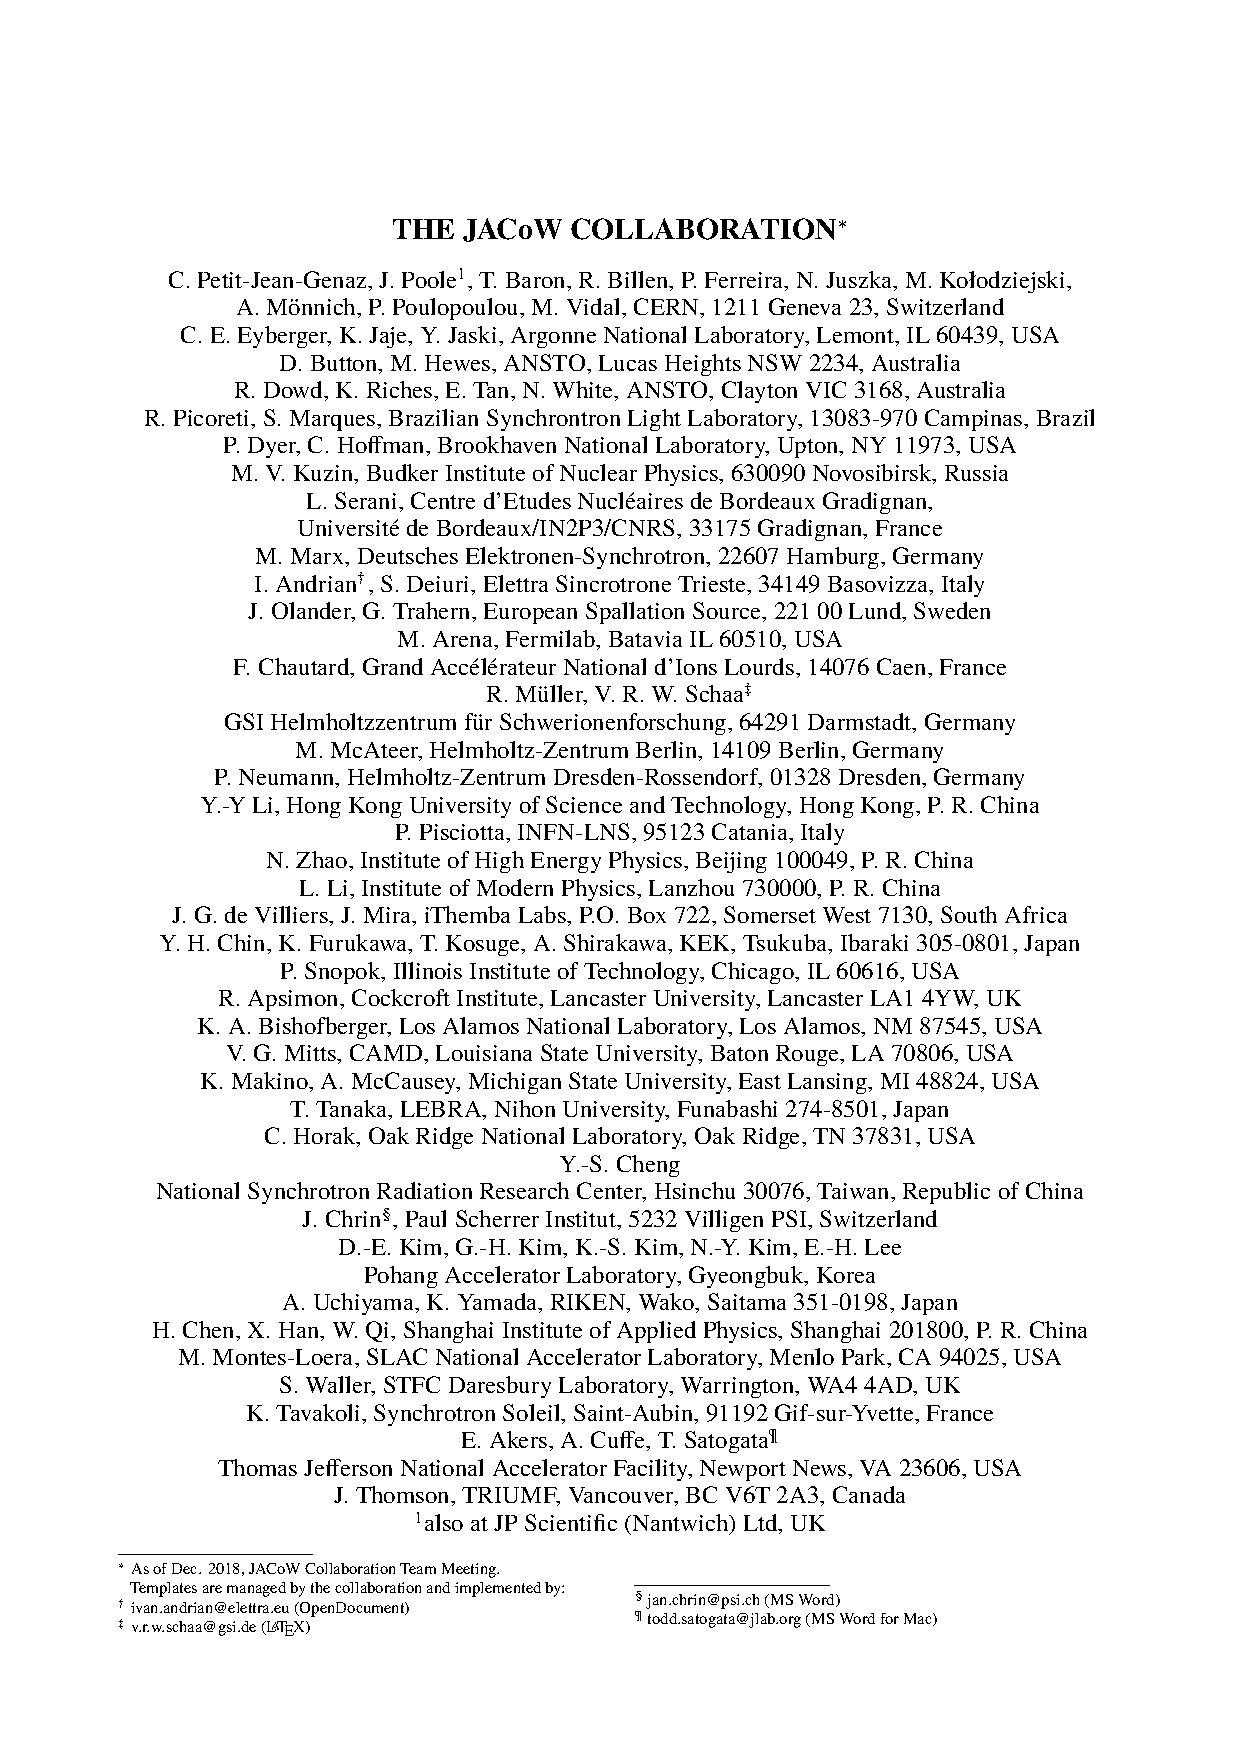
\includepdf[pages=-, noautoscale, pagecommand={}]{jacow-collaboration.pdf}{}

\clearpage

\twocolumn[\vspace*{-1.8ex}\section{ANNEX B:\endgraf IEEE REFERENCE STYLE GUIDE AS APPLIED TO \NoCaseChange{JACoW} PAPERS, \break PERIODICALS AND OTHER WORKS}\vspace*{\baselineskip}]

\subsection{Referencing JACoW Proceedings}

The format for published JACoW proceedings papers is detailed in the following 
and can also be readily deduced from Refs.~[1-3]. At the very minimum, sufficient 
information should be given to enable readers to clearly identify the paper and 
to facilitate its import into digital databases.
\vspace*{-.6\baselineskip}

\subsubsection{Author Listing} Careful attention should be given to the
placing of commas and the use of ‘and’ in the author list.
In particular, for the case of three or more authors
(as in [3]), a comma also follows the penultimate author.
The preference for ‘\emph{et al.}’\ takes precedence when the number
of authors becomes large (e.g., $>$6).
\vspace*{-.6\baselineskip}

\subsubsection{Paper Title} As is modern practice in references, the title
of the paper is written in sentence case, i.\,e., only the
initial letter of the first word in the title is capitalized.
Proper nouns, however, also have a capital. Capital letters
appearing in acronyms likewise remain unaltered
\vspace*{-.6\baselineskip}

\subsubsection{Conference Proceedings} The title of the proceedings is
written in title case in italics using standard abbreviations,
such as \emph{Int.} and \emph{Conf.} The preposition, ``in'', in normal
font, precedes the proceedings title. The location,
i.\,e., city, state (if USA), and country of the conference
venue, the month (three-letter abbreviation) and the year
the conference took place, is then listed. Finally, details
pertaining to the paper itself, such as the conference paper
ID, mandatory page numbers, and the digital object
identifier (DOI), if existing, are listed in the given order.
A monospaced font for the DOI is used so as to help
distinguish it from normal text. In \LaTeX{}
the ‘url’ package is used. The Word template uses the Liberation
Mono TrueType font (size 8 pt), or Lucida Sans Typewriter
font (size 7.5 pt) in earlier Word versions where the Liberation
Mono font may not be available. In LaTeX, the ‘url’
package is used with its default font now being switched to 
``newtxtt'' which offers a better distinction between 
``\texttt{O}'' and ``\texttt{0}''. The conference
paper ID is optional and may be included in the absence
of a DOI to facilitate a search through internet search
engines. DOIs have been assigned to all JACoW
publications appearing in recent proceedings and will
likewise be assigned to articles from conferences further
past, in due course. The use of DOIs is strongly
emphasized.

The complete or abbreviated form for citations, as
shown in the following section, is advocated. The former
is more informative to readers outside the immediate
conference sphere, and will further serve to avoid
potential ambiguities in cases where an acronym is not
unique. Both forms, however, when adhered to, ensure a
proper import into digital libraries and information
sources such as INSPIRE, Scopus, and Google Scholar.
Authors are also reminded to make a distinction between
papers published in JACoW proceedings (which have
page numbers and, in the case of recent publications,
DOIs) and those papers that may have been presented at
past JACoW conferences but were not published~[4].
References to contributions presented at the same
conference should be written as shown in [5]; the wording
“this conference” may be optionally appended.

\subsection{Referencing Periodicals and Other Sources}

The IEEE style is also shown for periodicals [6-11],
online sources [12], books [13, 14], internal reports [15],
theses [16], manuals or handbooks [17], patents [18] and
unpublished material [19, 20]. When citing a periodical,
only the official abbreviation of the journal should be used
[21]. Examples of correctly formatted references can also be 
found at the JACoW website, under ‘Formatting Citations’ which 
is reached through the ‘for Authors’ link.

\subsection{Alignment of References}

In the \LaTeX{} template, \verb|\bibliography{9}| is used for
when the total number of references is less than ten. This
should be changed to \verb|\bibliography{99}| if the number of
references is ten or more.

\patchcmd\thebibliography{\section*{REFERENCES\@mkboth {REFERENCES}{REFERENCES}}}{}{}{}
\section{PAPER PUBLISHED IN A CONFERENCE PROCEEDINGS}

\definecolor{jgreen}{cmyk}{0.81, 0.00, 0.97, 0.00}
\definecolor{jred}{cmyk}  {0.00, 0.99, 1.00, 0.00}
\definecolor{jgrepc}{cmyk}{0.74, 0.05, 1.00, 0.00}
\definecolor{jblue}{cmyk} {0.87, 0.54, 0.00, 0.00}
\definecolor{jvio}{cmyk}  {0.41, 0.82, 0.00, 0.00}
\definecolor{jbook}{cmyk} {0.28, 0.88, 0.79, 0.25}
\definecolor{jrept}{cmyk} {0.07, 0.70, 1.00, 0.00}
\definecolor{jmanu}{cmyk} {0.28, 0.77, 1.00, 0.23}
\definecolor{junpu}{cmyk} {0.00, 0.83, 0.65, 0.00}


\subsection{Complete Form}

\newcommand{\CCom}[2]{\newline\textcolor{#1}{[#2]}}
%\begin{thebibliography}{99}   % Use for  10-99  references
\begin{thebibliography}{9} % Use for 1-9 references
	
	\bibitem{item:1-1}
	A.~Alpha and B.~T.~Beta, “Novel techniques for future TeV electron accelerators”,
	in \textit{Proc.\ 9th Int.\ Particle Accelerator Conf.\ (IPAC’18)},
	Vancouver, BC, Canada, Apr.-May 2018.
	pp. 567-569. \url{doi:10.18429/JACoW-IPAC2017-PAPERID}
	\CCom{jgreen}{Conference Proceedings, two authors; DOI encouraged}

	\bibitem{item:1-2}
	A.~Alpha \emph{et al.},
	“A novel injector”, in \emph{Proc.\ 29th Linear Accelerator Conf.\ (LINAC’18)},
	Shanghai, China, Sep.\ 2018, pp.\ 27-31. %\newline
	\url{doi:10.18429/JACoW-LINAC2018-PAPERID}
	\CCom{jgreen}{Conference Proceedings, for six or more authors use \emph{et al.};	
		 DOI encouraged}
	
	\bibitem{item:1-3}	
	A.~Alpha, B.~T.~Beta, C.~Gamma, and D.~Delta,
	“An overview of control systems”,
	in \emph{Proc.\ 13th Int.\ Conf.\ on Accelerator and Large Experimental Physics Control Systems (ICALEPCS’11)}, Grenoble, France, Oct.\ 2011,
	paper TUP014, pp.\ 89--91.
	\CCom{jgreen}{Conference Proceedings, four authors; optional paper ID
	in the absence of a DOI}
\end{thebibliography}

\vspace*{-.5\baselineskip}
\subsection{Abbreviated Form}

\begin{thebibliography}{9} % Use for 1-9 references
	\bibitem{item:2-1}
	A.~Alpha and B.~T.~Beta, “Novel techniques for future TeV electron accelerators”,
	in \textit{Proc.\ IPAC’18}, 	Vancouver, BC, Canada, Apr.-May 2018,
	pp.\ 567-569. %\newline
	\url{doi:10.18429/JACoW-IPAC2018-PAPERID}
	\CCom{jgreen}{Conference Proceedings, two authors; DOI encouraged}
	
	\bibitem{item:2-2}
	A.~Alpha \emph{et al.},
	“A novel injector”, in \emph{Proc.\ LINAC’18},
	Shanghai, China, Sep.\ 2018, pp.\ 27-31. %\newline
	\url{doi:10.18429/JACoW-LINAC2018-PAPERID}
	\CCom{jgreen}{Conference Proceedings, for six or more authors use \emph{et al.}; DOI encouraged}
	
	\bibitem{item:2-3}	
	A.~Alpha, B.~T.~Beta, C.~Gamma, and D.~Delta,
	“An overview of control systems”,
	in \emph{Proc.\ ICALEPCS’11}, Grenoble, France, Oct.\ 2011,
	paper TUP014, pp.\ 89--91.
	\CCom{jgreen}{Conference Proceedings, four authors; optional paper ID
				  in the absence of a DOI}
\end{thebibliography}

\section{UNPUBLISHED PAPER PRESENTED AT A PREVIOUS CONFERENCE}

\subsection{Complete Form}

\begin{thebibliography}{9} % Use for 1-9 references
\setcounter{enumi}{3}
 \bibitem{item:41}
	A.~Alpha and B.~T.~Beta,
	“An interesting talk but paper not submitted”,
	presented at the 5th Int.\ Particle Accelerator Conf.\ (IPAC’14),
	Dresden, Germany, Jun.\ 2014, paper MOAX01, unpublished.
	\CCom{jred}{Unpublished paper; conference name in normal font; paper
	ID may only be given if material supplementing the proceedings
	exists on the JACoW website, e.\,g., PDF of talk}
\end{thebibliography}

\subsection{Abbreviated Form}

\begin{thebibliography}{9} % Use for 1-9 references
\setcounter{enumi}{3}
 \bibitem{item:42}
	A.~Alpha and B.~T.~Beta,
	“An interesting talk but paper not submitted”,
	presented at IPAC’14,
	Dresden, Germany, Jun.\ 2014, paper MOAX01, unpublished.
	\CCom{jred}{Unpublished paper; conference name in normal font; paper
	ID may only be given if material supplementing the proceedings
	exists on the JACoW website, e.\,g., PDF of talk}
\end{thebibliography}


\section{PAPER PRESENTED AT THE CURRENT CONFERENCE}

\subsection{Complete Form}

\begin{thebibliography}{9} % Use for 1-9 references
\setcounter{enumi}{4}
 \bibitem{item:51}
	A.~Alpha and B.~T.~Beta,
	“An interesting talk at this conference”,
	presented at the 10th Int.\ Particle Accelerator
	Conf.\ (IPAC’19), Melbourne, Australia, May 2019, 
	paper MOAB01, this conference.
	\CCom{jgrepc}{Current conference; conference name in normal font; 
				  the wording “this conference” is optional}
\end{thebibliography}

\subsection{Abbreviated Form}

\begin{thebibliography}{9} % Use for 1-9 references
\setcounter{enumi}{4}
	\bibitem{item:52}
	“An interesting talk at this conference”,
	presented at IPAC’19, Melbourne, Australia, May 2019, 
	paper MOAB01, this conference.
	\CCom{jgrepc}{Current conference; conference name in normal font; 
				  the wording “this conference” is optional}
\end{thebibliography}


\vspace*{-.5\baselineskip}
\section{PAPER PUBLISHED IN, OR SUBMITTED TO, A PERIODICAL}

\begin{thebibliography}{99} % Use for 1-9 references
  \setcounter{enumi}{5}
	\bibitem{item:6}
		P.~Mercury \emph{et al.},
		“Title of paper published in journal”,
		\emph{Phy.\ Rev.\ Lett.}, vol.\ 114, no.\ 5,
		p.\ 050511, Feb.\ 2014.
		\url{doi:10.1103/PhysRevLett.114.050511}
	\CCom{jblue}{Periodical, Phys.\ Rev.\ Lett.;
		             issue no.\ and month may be omitted}

	\bibitem{item:7}
		P.~Venus \emph{et al.},
		“New techniques in laser wakefield accelerators”,
		\emph{Phys.\ Rev.\ ST Accel.\ Beams}, vol.\ 18,
		p.\ 120198, Dec.~2015. %\newline
		\url{doi:10.1103/PhysRevAccelBeams.18.120198} 
	\CCom{jblue}{Periodical, Phys.\ Rev.\ ST Accel.\ Beams;
			              month may be omitted}

	\bibitem{item:8}
		T.~Earth \emph{et al.},
		“Low dose irradiation impact on modern silicon detectors”,
		\emph{Nucl.\ Instr.\ Meth.}, vol.\ 692, pp.\ 256--280, 2014.
		\url{doi:10.1016/j.nima.2014.11.022}
	\CCom{jblue}{Periodical, Nucl. Instr. Method.}
	
	\bibitem{item:9}
		T.~Earth, L.~Moon, and A.~Belt,
		“Temporal correlations of x-ray free electron lasers”,
		\emph{Optics Express}, vol.\ 20, pp.\ 11396--11404, 2012.
		\url{doi:10.1364/OE.20.11396}
	\CCom{jblue}{Periodical, Optics Express}

	\bibitem{item:10}
		J.~B.~Good,
		“A paper accepted for publication”,
		\emph{Phys.\ Rev.\ Lett.}, to be published.
	\CCom{jblue}{Periodical, paper accepted for publication
		              by Phys. Rev. Lett.}

	\bibitem{item:11}
		G.~D.~Read,
		“Title of paper submitted for publication”,
		submitted for publication.
	\CCom{jblue}{Paper submitted for publication; the name of the
					  periodical does not appear}
\end{thebibliography}

\vspace*{-.5\baselineskip}
\section{ONLINE SOURCE}

\begin{thebibliography}{99} % Use for 1-9 references
  \setcounter{enumi}{11}
	\bibitem{item:121}
		JACoW, \url{http://www.jacow.org} 
		\CCom{jvio}{online source; no hyperlink, no period at end of URL unless there is a trailing “/” as shown below. A monospaced font should be used, this is achieved using the ‘url’ package in \LaTeX}

  \setcounter{enumi}{11}
	\bibitem{item:122}
		JACoW, \url{http://www.jacow.org/}.  
		\CCom{jvio}{online source; no hyperlink, period after trailing “/” in URL
					if optionally preferred. A monospaced font should be used, this is
					achieved using the ‘url’ package in \LaTeX}

\end{thebibliography}

\section{CITATIONS TO BOOKS}

\begin{thebibliography}{99} % Use for 1-9 references
	\setcounter{enumi}{12}
	\bibitem{item:13}
		T.~Earth and L.~Moon,
		“Title of chapter in the book”,
		in \emph{Title of Book}, R Mars, Ed.\ New York, NY, USA:
		Wiley, 1994, pp.\ 42--48. 
	\CCom{jbook}{Chapter in book}
	
	\bibitem{item:14}
		A.~Belt, \emph{Title of Book}. Cambridge, MA, USA:
		MIT Press, 1986. 
	\CCom{jbook}{Book}
\end{thebibliography}

\section{REPORTS AND THESES}

\begin{thebibliography}{99} % Use for 1-9 references
	\setcounter{enumi}{14}
	\bibitem{item:15}
		G. Jupiter \emph{et al.},
		“Title of report”, CERN, Geneva, Switzerland,
		Rep.\ CERN-2012-333, Oct.\ 2012.
	\CCom{jrept}{Report}

	\bibitem{item:16}
		A.~Student, “Title of thesis”,
		Ph.D.\ thesis, Phys.\ Dept.,
		Karlsruher Institut für Technologie, Karlsruhe,
		Germany, 2014.
	\CCom{jrept}{Thesis}
\end{thebibliography}

\section{MANUAL}

\begin{thebibliography}{99} % Use for 1-9 references
	\setcounter{enumi}{16}
	\bibitem{item:17}
		\emph{IEEE Editorial Style Manual},
		IEEE Periodicals,
		Piscataway, NJ, USA, Oct.\ 2014, pp.\ 34-52;
		\url{http://www.ieee.org/documents/style_manual.pdf} 
	\CCom{jmanu}{Handbook/Manual, no hyperlink, no period after URL}
\end{thebibliography}

\section{PATENTS}

\begin{thebibliography}{99} % Use for 1-9 references
	\setcounter{enumi}{17}
		\bibitem{item:18}
		A.~N.~Inventor,
		“Title of patent”,
		Patent Authority and No., Jan.\ 20, 2016.

\end{thebibliography}

\section{UNPUBLISHED WORK AND PRIVATE COMMUNICATION}

\begin{thebibliography}{99} % Use for 1-9 references
	\setcounter{enumi}{18}
	\bibitem{item:19}
		P.~Neptune, “Title of paper”, unpublished.
	\CCom{junpu}{Unpublished}
	
	\bibitem{item:20}
	P.~Uranus, private communication, Jun.\ 2015.
	\CCom{junpu}{Private communication}
\end{thebibliography}

\newpage

\section{JOURNAL ABBREVIATIONS}

\begin{thebibliography}{99} % Use for 1-9 references
	\setcounter{enumi}{20}
	\bibitem{item:21}
		\url{https://woodward.library.ubc.ca/researchhelp/journal-abbreviations/}

\end{thebibliography}

\newpage

\twocolumn[\vspace*{-1.8ex}\section{ANNEX C:\endgraf THE DILIGENT AUTHOR’S CHECKLIST}\vspace*{\baselineskip}]
\flushcolsend

\subsection{Common Oversights}

In order to lessen the load on a small team of editors
and to help expedite publication of the Proceedings, authors
are kindly asked to give themselves an extra few
minutes to go over the following points, which highlight
the most common errors, before uploading their paper. By
providing a properly formatted JACoW paper, the Proceedings
Office is able to benefit from an autodistill process
which automatically converts the author's PDF file
into a version that adheres to the JACoW-compliant PDF
standard. The process further ensures that all fonts required
to view the entire document are embedded, rendering
a final PDF that qualifies technically for publication.


\subsection{Author and Affiliation Listing}

The names of authors and their affiliations should be in
\SI{12}{pt} uppercase and lowercase letters, with standard,
roman fonts (i.\,e., not italics). When there is more than
one author, the submitting author should be first, followed
by the coauthor. Coauthors should be grouped by affiliation
and then be listed alphabetically. Please refer to \textbf{ANNEX~A}
for further details and examples, particularly for
the case where authors have multiple institutes.

\subsection{SPMS Database and Final Manuscript Validation}

Primary authors are reminded that it is their
responsibility to verify the accuracy of the title, abstract,
and coauthor/institute listing, and that these are identical
in both the final manuscript and SPMS database. This is
required to ensure the proper indexing of author/coauthor(s) 
appear in the published proceedings.

\subsection{Subsection Headings}

Subsection Headings are in \SI{12}{pt} \emph{italic} lowercase and uppercase.
The initial letter of every principle word is capitalized,
and the heading is left aligned in the column.

\subsection{Figure Captions}

Figure captions should be placed \emph{below} the figure and
centred if on one line, but justified if spanning two or
more lines:
\begin{center}
	Figure 1: A one line figure caption is centred.
\end{center}
\begin{justify}
	Figure 2: A lengthy figure caption that spans
	two lines is justified.
\end{justify}

Note the colon “:” after the figure number and the period
“.” at the end of the caption.

When referring to a figure from within the text, the
convention is to use the abbreviated form, i.\,e., Fig.~1,
\emph{unless} the reference to the figure is at the start of the sentence:
\begin{quote}
	Figure 1 shows a schematic view of\ldots
	
	\ldots as shown in Fig.~1.
\end{quote}

% if set as \subsection, the title will appear at the top
% of the column followed by "Table captions ... lines:", 
% then follows the text above after the justify till end of quote
\iffalse
\subsection{Table Headings}
\else
\noindent\textit{\vspace{1em}\large Table Headings}
\fi

Table captions should be placed \emph{above} the table and
centred if on one line, but justified if spanning two or
more lines:
\begin{center}
	Table 1: Table Heading
\end{center}

\begin{justify}
	Table 2: A Particularly Long Table Heading
	Spanning Two Lines
\end{justify}

Note the colon “:” after the table number, that the initial
letters of the principle words in the table heading are
capitalized, and the absence of a period at the end of the
caption.

When referring to a table from within the text, the convention
is \emph{not} to abbreviate, i.\,e., Table 1.

\subsection{Equations}

If a displayed equation requires a number, it should be
placed flush with the right margin of the column. 

\subsection{Units}

An unbreakable space should always precede a unit. In \LaTeX{} use
a “\verb|\,|” or the ‘siunitx’ package to format units.
Examples are:
\SI{3}{keV}, \SI{4}{GeV}, \SI{100}{kW}, \SI{7}{\micro m}.

\subsection{References}

References are written in \SI{9}{pt} size and should be neatly
presented in a consistent format with reference numbers
aligned. Please refer to \textbf{ANNEX~B} for the preferred format
and proper alignment.

Please also ensure that references in the text are cited in
sequential order.

\flushend


\end{document}
